\begin{table}[t]
\centering
\caption{Task 2 specialist training snapshot on all 736 validation IDs (7,360 fixed cases). Each specialist is applied only to its corresponding corruption, with identity on the other three classes. These are validation selection scores, not routed test scores.}
\label{tab:specialist-snapshot}
\begin{tabular}{lrr}
\toprule
Specialist & Best epoch & Validation score $\downarrow$ \\
\midrule
Salt-and-pepper & 39 & 0.06177 \\
Gaussian blur & 13 & 0.09243 \\
Occlusion & 13 & 0.07955 \\
\bottomrule
\end{tabular}
\end{table}

The salt specialist completed its 40-epoch fit. The blur and occlusion values in Table~\ref{tab:specialist-snapshot} are checkpoint snapshots while their full fits continue. A matched, smaller validation comparison of complete routing behavior appears in Table~\ref{tab:routing-snapshot}.

\begin{table}[t]
\centering
\caption{Matched restoration comparison on the first 32 validation IDs, each with ten deterministic cases (320 cases total). MAE and SSIM average the ten condition/severity cells equally. This is preliminary validation evidence, not official-test performance.}
\label{tab:routing-snapshot}
\begin{tabular}{lrrr}
\toprule
System & MAE $\downarrow$ & SSIM $\uparrow$ & Score $\downarrow$ \\
\midrule
Damaged input & 0.05099 & 0.66688 & 0.10741 \\
Hard oracle & 0.03581 & 0.81737 & 0.06517 \\
Hard predicted & 0.03580 & 0.81796 & 0.06505 \\
Soft mixture & 0.03579 & 0.82157 & 0.06432 \\
\bottomrule
\end{tabular}
\end{table}

The classifier chose the correct label in 319 of the 320 matched cases (99.69\% accuracy, 0.9948 macro-F1). The predicted route's small score advantage over the oracle on this subset is not evidence that misrouting helps generally: one occlusion case was sent through identity, and a different output can score better by chance. The hard-versus-soft score difference is only 0.00073 here and does not establish a reliable ranking outside this subset.

\begin{table}[t]
\centering
\caption{Task 3 short-fit validation evidence, using 32 validation IDs (320 fixed cases), 20 training steps per epoch, and the Task 2 checkpoint snapshots. This smaller subset is not comparable to full-validation or held-out test scores.}
\label{tab:soft-snapshot}
\begin{tabular}{lrr}
\toprule
Epoch & Validation score $\downarrow$ & Training loss \\
\midrule
0 (gate warm-up) & 0.05424 & 0.12029 \\
1 (joint tuning) & 0.05056 & 0.10538 \\
2 (joint tuning) & 0.05195 & 0.10614 \\
\bottomrule
\end{tabular}
\end{table}

The Task 3 gate's selected epoch-1 model assigns mean weight 0.998 to the identity branch on clean cases and 0.9999 to the noise branch on noisy cases in this 32-ID validation subset. For blur, it assigns 0.853 to the blur expert and 0.147 to identity; for occlusion, it assigns 0.911 to the occlusion expert and 0.088 to identity. These weights show interpretable short-run specialization, but the limited subset cannot establish final generalization.

\begin{figure}[t]
\centering
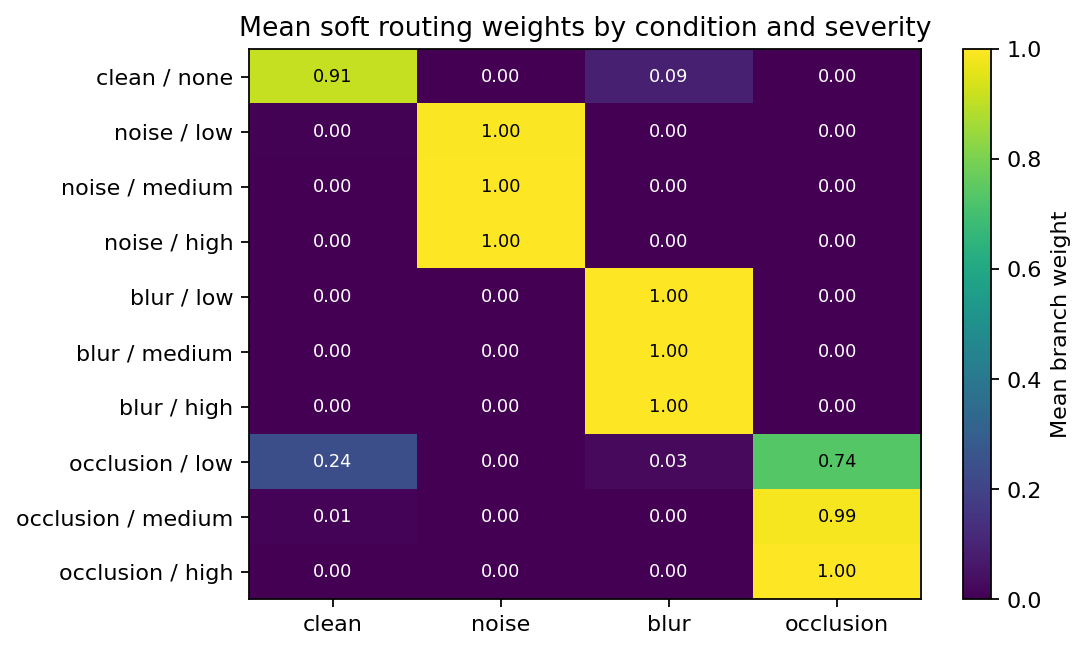
\includegraphics[width=\columnwidth]{figures/task3_submission_routing_heatmap.png}
\caption{Soft-gate mean weights on the same 320 preliminary validation cases, grouped by true corruption and severity. The figure uses the epoch-0 snapshot exported to ONNX for the application.}
\label{fig:task3-submission-weights}
\end{figure}
